\documentclass[12pt]{article}

\usepackage[utf8]{inputenc}
\usepackage{setspace}
\usepackage{geometry}
\usepackage{graphicx}
\usepackage{caption}
\usepackage{indentfirst}
\usepackage{anyfontsize}
\usepackage{textcomp}
\usepackage{mathtools}
\usepackage{float}
\usepackage{changepage}
\usepackage [english]{babel}
\usepackage [autostyle, english = american]{csquotes}
\usepackage{tabto}
\usepackage{verbatim}
\usepackage{wrapfig}
\usepackage{caption}
\usepackage{subcaption}
\usepackage{stackengine}
\usepackage{scrextend}
\usepackage{xcolor}
\usepackage{booktabs}
\usepackage{bigints}
\usepackage{calc}
\usepackage[nomessages]{fp}


\graphicspath{}
\MakeOuterQuote{"}

\title{Models with Delays}
\author{Geneva Porter}
\date{11 December 2018}

\begin{comment}

\begin{figure}[H]
\centering{\includegraphics[width=15cm]{FILENAME.eps}}
\caption*{\textbf{CAPTION}}
\end{figure}

$\left(\begin{matrix}
11      & 12  \\
21      & 22  \\
\end{matrix}\right)$

\begin{table}[]
\begin{center}
\begin{tabular}{|l|l|} \hline
&  \\ \hline
&  \\ \hline
\end{tabular}
\caption*{\textbf{} }
\end{center}
\end{table}

\end{comment}

\begin{document}
	
\begin{titlepage}
\maketitle
\thispagestyle{empty}


\begin{center}
	
\large \it San Diego State University 
	
Professor J Mahaffy, Math 636

\end{center}
\end{titlepage}

\section*{Goodwin Models for Genetic Expression}

The Goodwin models describe genetic regulation. They are given by:

\begin{center}
$\left(\begin{matrix}
{dm(t)}/{dt} \\
{dp(t)}/{dt}\\
{dr(t)}/{dt}
\end{matrix}\right)=
\left(\begin{matrix}
\dfrac{1}{1+r(t-k)^n}-b_1m(t) \\
m(t)-b_2p(t)\\
p(t)-b_3r(t)
\end{matrix}\right)$
\end{center}

In this model, $b_1$, $b_2$, and $b_3$ are decay constants, $k$ is the delay for transcription and translation, and $n$ is the Hill coefficient, which we will give a value of 4. The functions $m(t)$, $p(t)$, and $r(t)$ represent the concentration of mRNA, the protein formed from the mRNA, and the end product repressor created by the protein, respectively.

\subsection*{Genetic Repression in Bacteria}

Bacteria possess mechanisms that allow for genetic regulation in response to environmental changes. Regulatory molecules in bacteria can activate and attach to DNA near a specific group of genes, then either help or block the the expression of those genes. This determines weather or not the specific group of genes will be transcribed into mRNA and expressed or blocked from transcription and repressed.

A group of genes, or an operon, is repressible if they can be "turned off" by a corepressor molecule. One example of this is the $trp$ operon found in {\it E. coli} bacteria, which facilitates the creation of tryptophan. When there are high levels of tryptophan present, the tryptophan can act as a corepressor and "turn off" the $trp$ operon. Likewise, when tryptophan levels are low, there is little repressor activity and the $trp$ operon can be "turned on" or activated to allow the biosynthetic production of the needed tryptophan.

The Goodwin model can be applied to $trp$ operon repression by examining the cyclical nature of the genetic repression-expression feedback loop found in bacteria. Let's say that low levels of tryptophan are present and the $trp$ operon is active. The operon continues to signal tryptophan synthesis through transcription to mRNA, and little repression is occuring because tryptophan is needed. As more synthesis occurs, the concentration of mRNA increases, and eventually a high level of tryptophan will facilitate the repression of $trp$. As tryptophan is used up by the bacteria, more will be needed. If the there is none available in the environment, repression of $trp$ ceases so that tryptophan can again be produced. 

The equations above describe this cycle. As the concentration of mRNA  increases, the rate of mRNA production $dm/dt$ decreases due to the term $-b_1m(t)$. The increased presence of repressor proteins also slows the rate of mRNA production, as seen in the first term of $dm/dt$. High amounts of mRNA means an increased rate of protein production, seen in the first term of $dp/dt$. As the population of proteins increase, its production rate slows, as indicated by the $-b_2p(t)$ term. The rate of change of the repressor created by the proteins ($dr/dt$) increases along with the $p(t)$ term when high levels of proteins are present, but decreases along with the $-b_3r(t)$ term as more repressors are produced. Decreasing amount of repressor proteins increases the the rate of mRNA production, and the cycle begins again.

\subsection*{Stability Analysis: Undelayed}

We can examine the Goodwin models with the parameter values $k=0$, $b_1=1$, $b_2=0.1$, and $b_3=0.05$. Setting the system to (0,0,0) with these parameters, we get a singe real equilibrium at $(e_m, e_p, e_r) = (0.08934, 0.89340, 1.78681)$. Taking the partial derivatives of each term to form the Jabobian matrix and plugging in the equilibrium values, we get:

\begin{center}
	$J\left(\begin{matrix}
	e_m      \\
	e_p      \\
	e_r      \\
	\end{matrix}\right)
	 = \left(\begin{matrix}
-1      & 0  	& -0.18213\\
1      & -0.1  	& 0\\
0      & 1  	& -0.5\\
\end{matrix}\right)\longrightarrow
\left(\begin{matrix}
\lambda_1     \\
\lambda_2      \\
\lambda_3      \\
\end{matrix}\right) = 
\left(\begin{matrix}
- 0.18806 - 0.39281i      \\
- 0.18806 + 0.39281i      \\
-1.22387      \\
\end{matrix}\right)$
\end{center}

The real part of each eigenvalue is negative, indicating that the equilibrium is stable at these parameters. The imaginary parts indicate that this equilibrium is a spiral node.

\subsection*{Stability Analysis: Delayed} 

If we include the delay term, our equilibrium remains the same, so $r(t-k)=r(t)$ at the equilibrium. However, the stability of the system at the equilibrium is more difficult to determine. Rather than taking the Jacobian (like for non-delay systems) and forming the characteristic equation from the determinant, we need to "separate" the delay term first. To accomplish this, we use the following form for our characteristic equation:

	$$\left|-\lambda I_l+J_0+\sum_{i=1}^{n}J_{\tau_i}e^{-\lambda\tau_i}\right|=0$$


Where $\lambda$ is the solution set of eigenvalues, $I_l$ is the identity matrix for a system of $l$ equations, $J_{\tau_i}$ is the Jacobian matrix (with respect to some delay $\tau_i$) evaluated at the equilibrium, and $n$ is the number of delays in the system. This gives us the characteristic equation of:


	$$\left|\left(\begin{matrix}
-1  -\lambda    & 0  	& -0.18213e^{-k\lambda}\\
1      & -0.1-\lambda   	& 0\\
0      & 1  	& -0.5-\lambda \\
\end{matrix}\right)\right|=0\hspace{5mm}\longrightarrow $$

$$\lambda^3+(1.6)\lambda^2+ (0.65)\lambda+(0.05) +(0.18213)e^{-\lambda k}=0$$

We can now examine the stability for delays of different values for $k$. Using MATLAB, I created a program to map the perimeter of the rectangle bound by the line $x=0$, $x=4$, $y=-3$, and $y=3$ under the transformation of the characteristic equation with $\lambda = x+iy$ (Appendix, Figure i). When separated in to real and imaginary parts, the characteristic equation is rather messy so it will not be shown here. The results are shown in Figures 1 and 2 below.

\begin{figure}[H]
	\centering{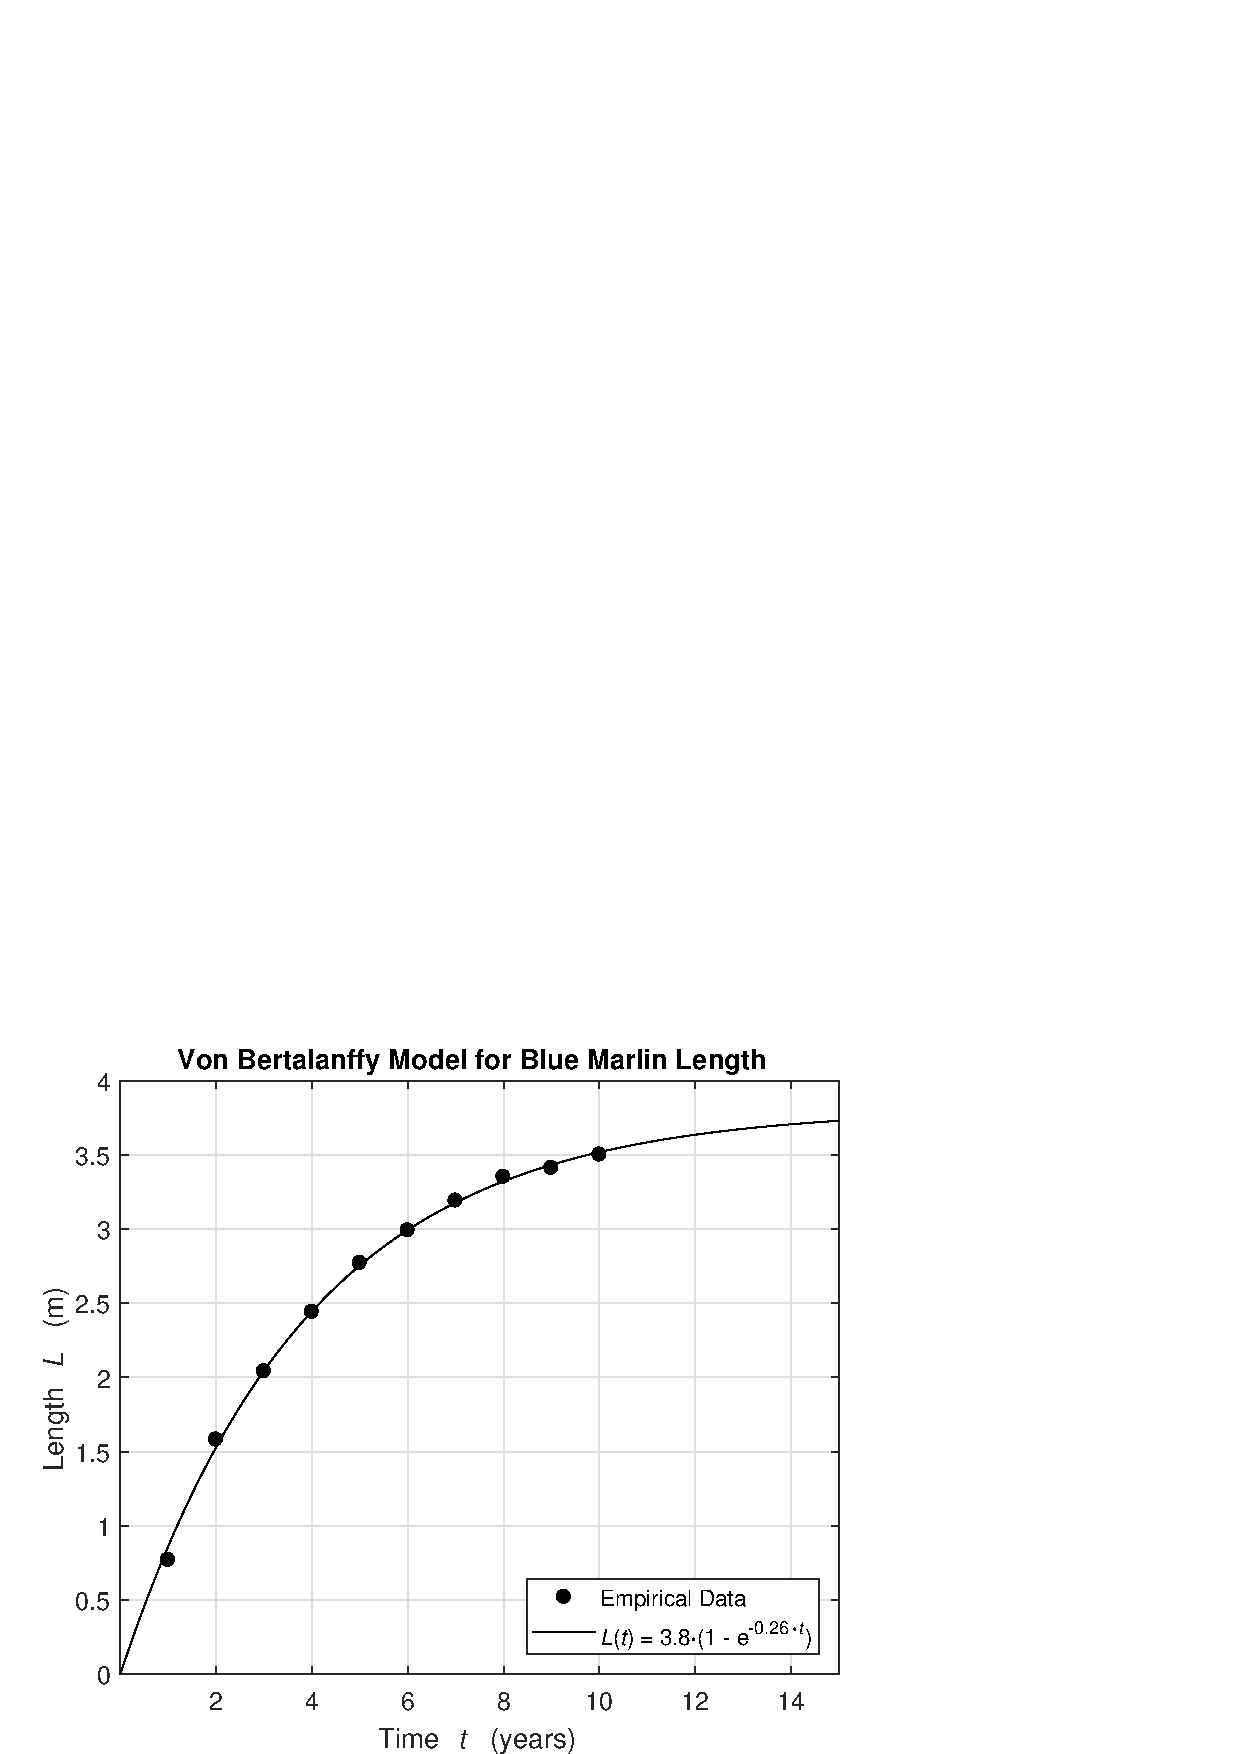
\includegraphics[width=14cm]{f3.png}}
	\caption*{\textbf{Figure 1} Transformation Under Characteristic Equation}
\end{figure}

\begin{figure}[H]
	\centering{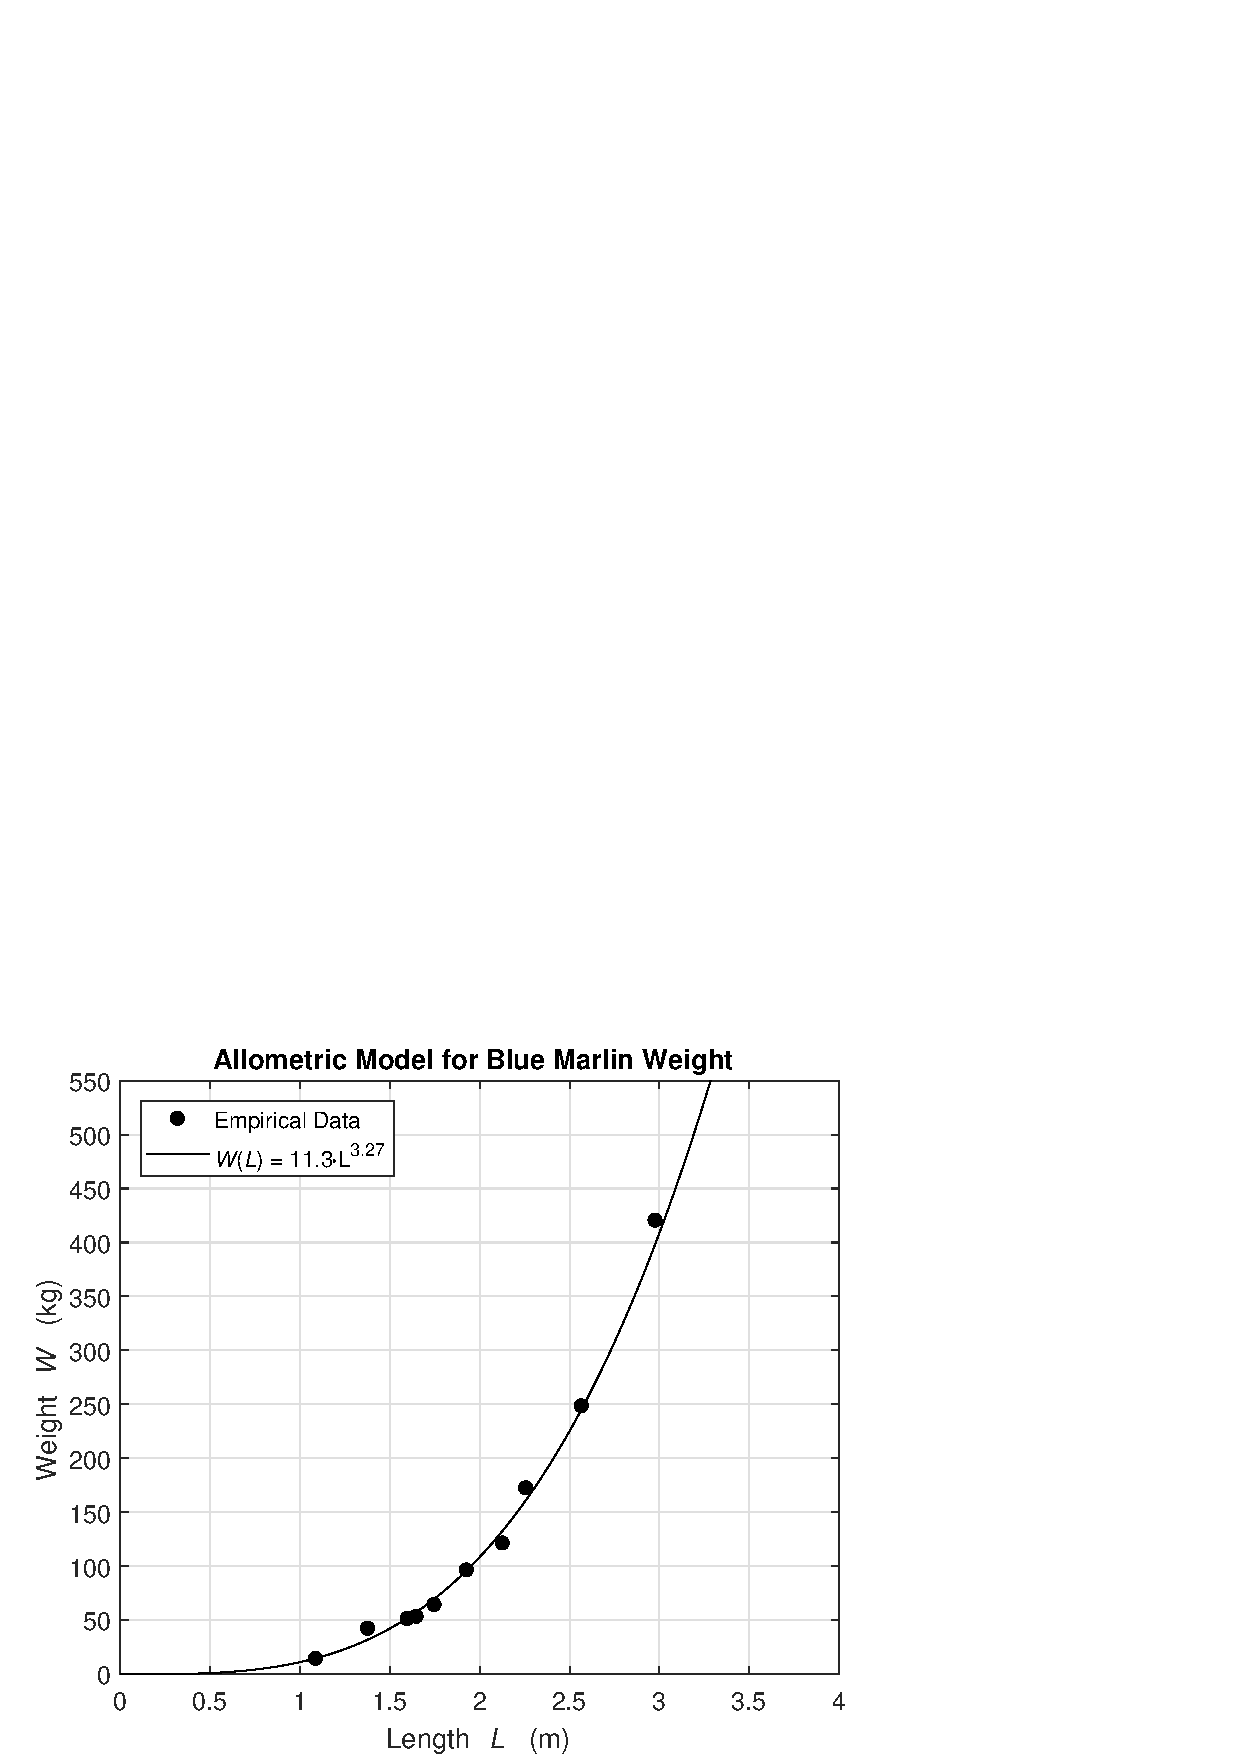
\includegraphics[width=14cm]{f4.png}}
	\caption*{\textbf{Figure 2} Differences Between $k=1$ and $k=4$}
\end{figure}

Examining these graphs, we can evaluate the winding number for each to determine how many eigenvalues lie inside the bounded region. For $k=1$, the winding number is 0. We can see from figure 1 that one counter-clockwise loop about the origin is made (+1), but the magnification in figure 2 shows that an additional loop appears going clockwise (-1). These add to zero, indicating that there are no eigenvalues contained in the region under this value of $k$. If we assume that this region is representative of all eigenvalues with positive real parts, then we can say that the system's eigenvalues likely have negative real parts, and the system is thus stable at the equilibrium we defined earlier.


For $k=4$, the winding number is 2. We have a similar loop in the clockwise direction (+1), and the magnification shows that the second loop is also in the clockwise direction (+1). Since these add to 2, there are 2 eigenvalues in the region we defined. This indicates that the system has 2 eigenvalues with positive real parts, and the equilibrium is likely unstable (or a saddle).

We can simulate the solutions to this model using MATLAB's function $dde23()$ (Appendix, figure ii). We assumed values of zero for each function for $t\leq0$. Figure 3 shows the results of the solutions for $k=1$ and $k=4$. Note that different historical values for the system resulted in similar long term behavior, indicating that the system is robust.

\begin{figure}[H]
	\centering{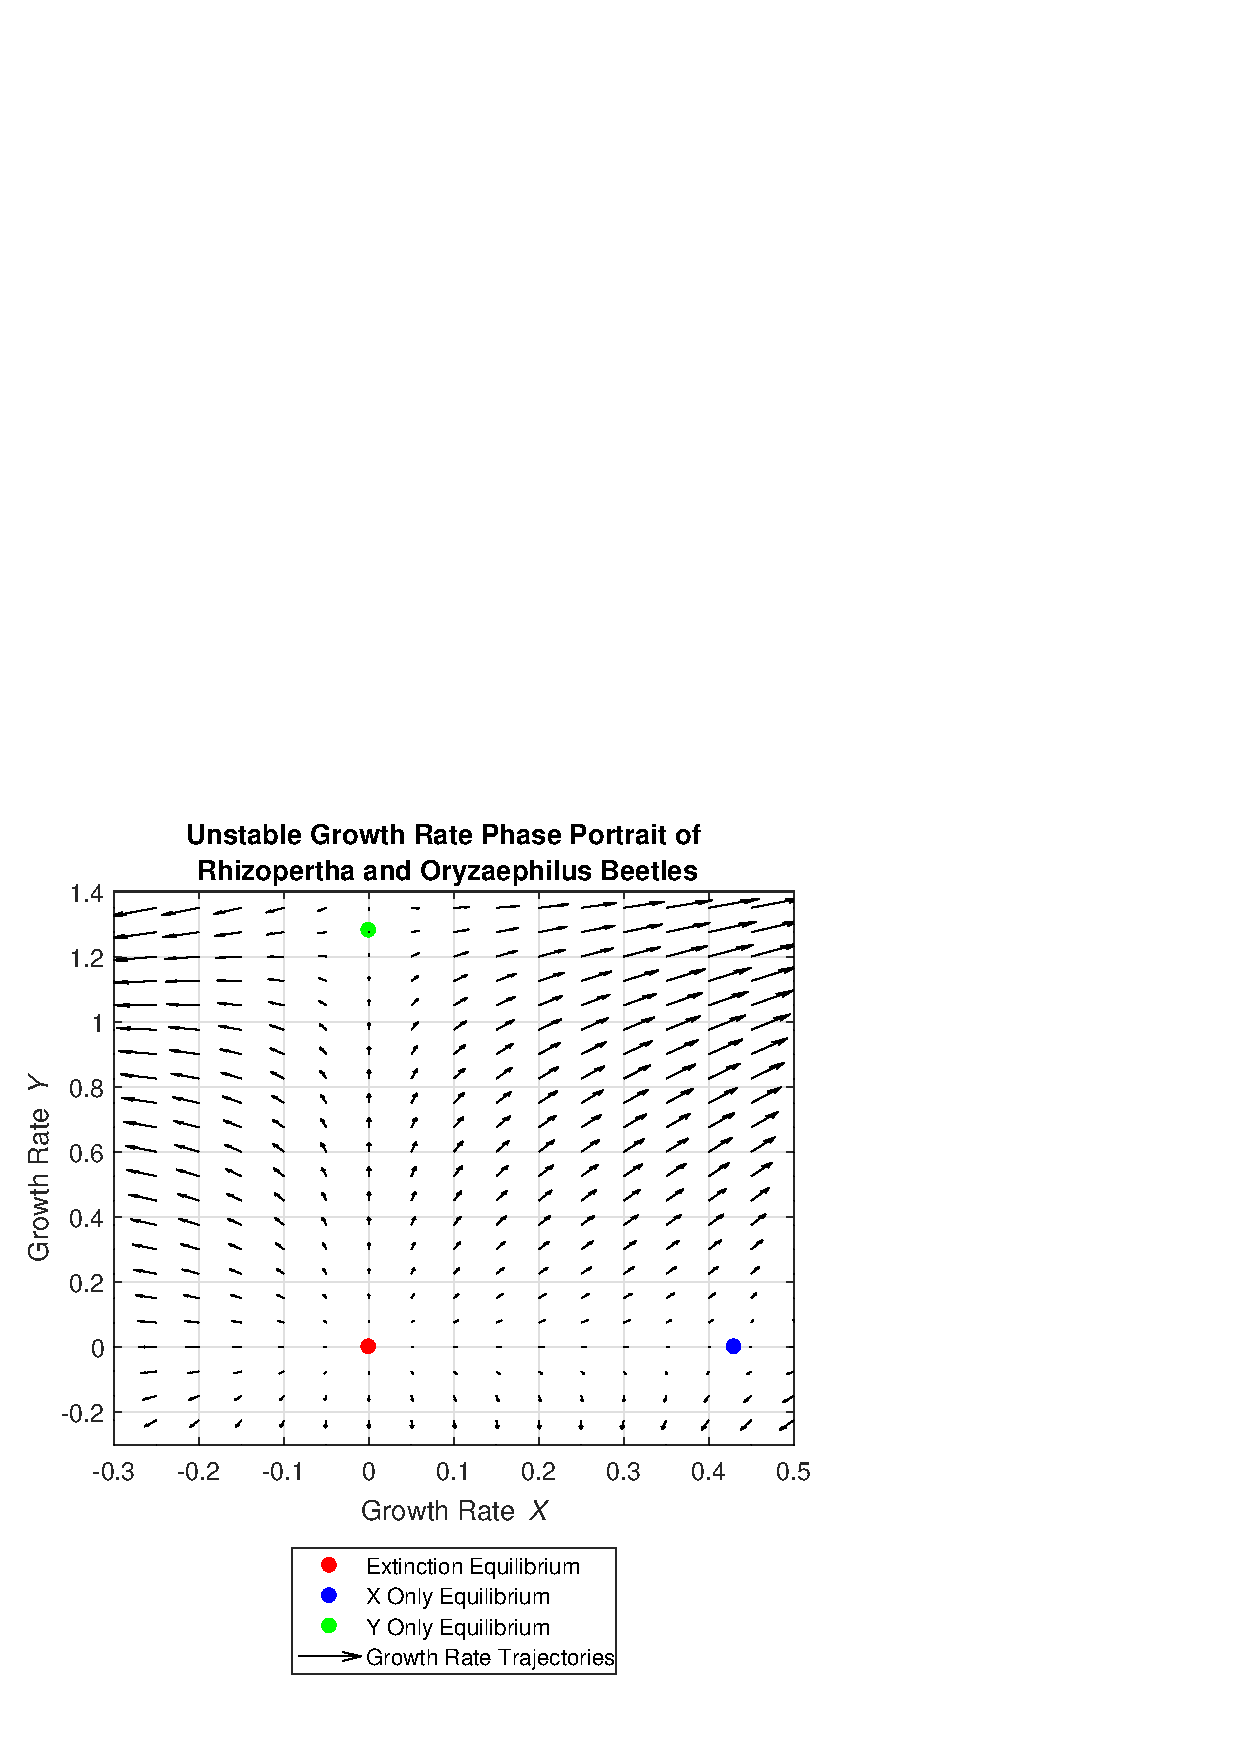
\includegraphics[width=14cm]{f7.png}}
	\caption*{\textbf{Figure 3} Differences Between $k=1$ and $k=4$}
\end{figure}

We can see here that the $k=1$ curves reach an equilibrium around $t=50$, and level off to smooth curves, indicating a stable equilibria. On the other hand, the $k=4$ curves oscillate about the equilibria for some time before smoothing out. 

\subsection*{Hopf Bifurcation}

We can find a Hopf bifurcation in this system by substituting $\lambda=i\omega$ into our characteristic equation, then setting both the real and imaginary parts equal to zero. MATLAB's $vpasolve()$ function was used to find the Hopf bifurcation values of $\omega=0.28680$ and $k=3.72894$. 

\pagebreak

\section*{Appendix}

\begin{figure}[H]
	\centering{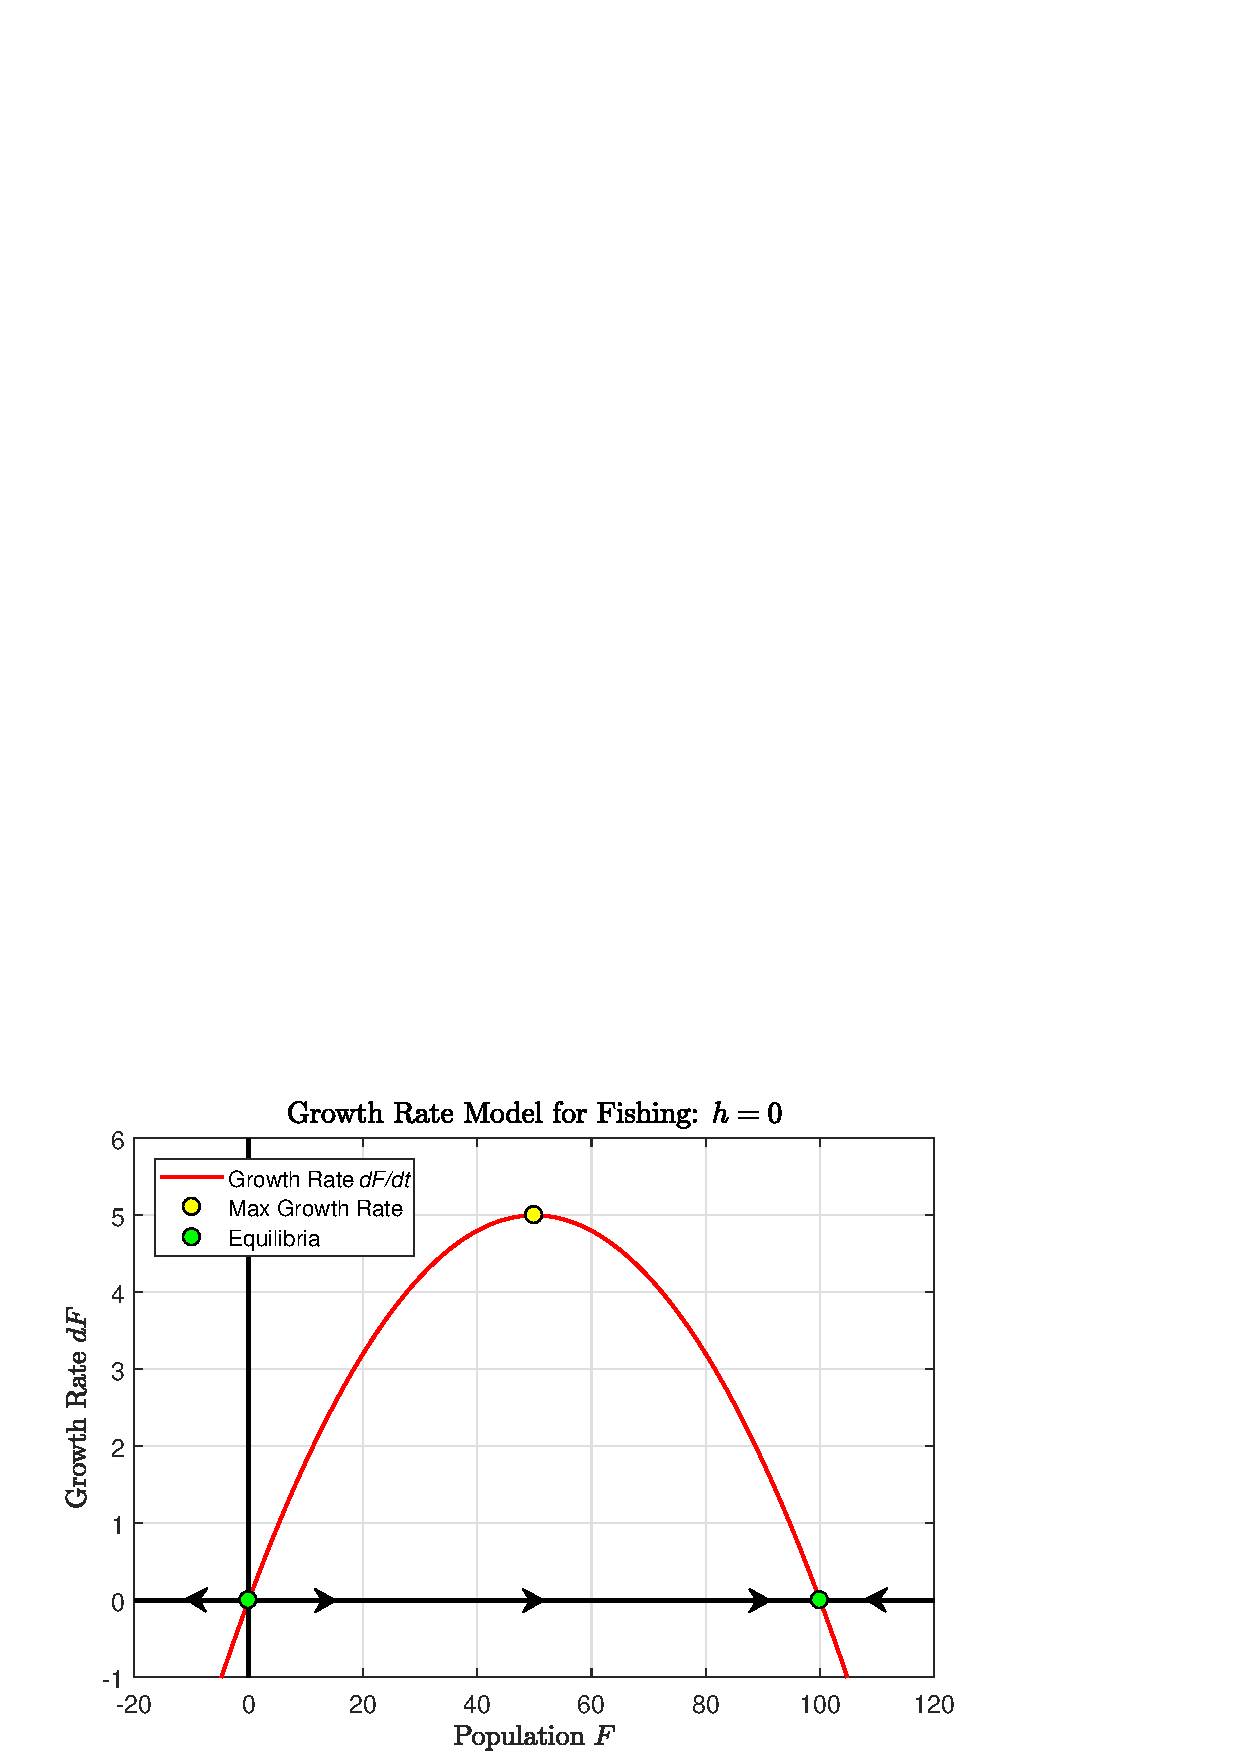
\includegraphics[width=13cm]{f1.png}}
	\caption*{\textbf{Figure i} MATLAB Code for Transformation via Characteristic Equation }
\end{figure}

\begin{figure}[H]
	\centering{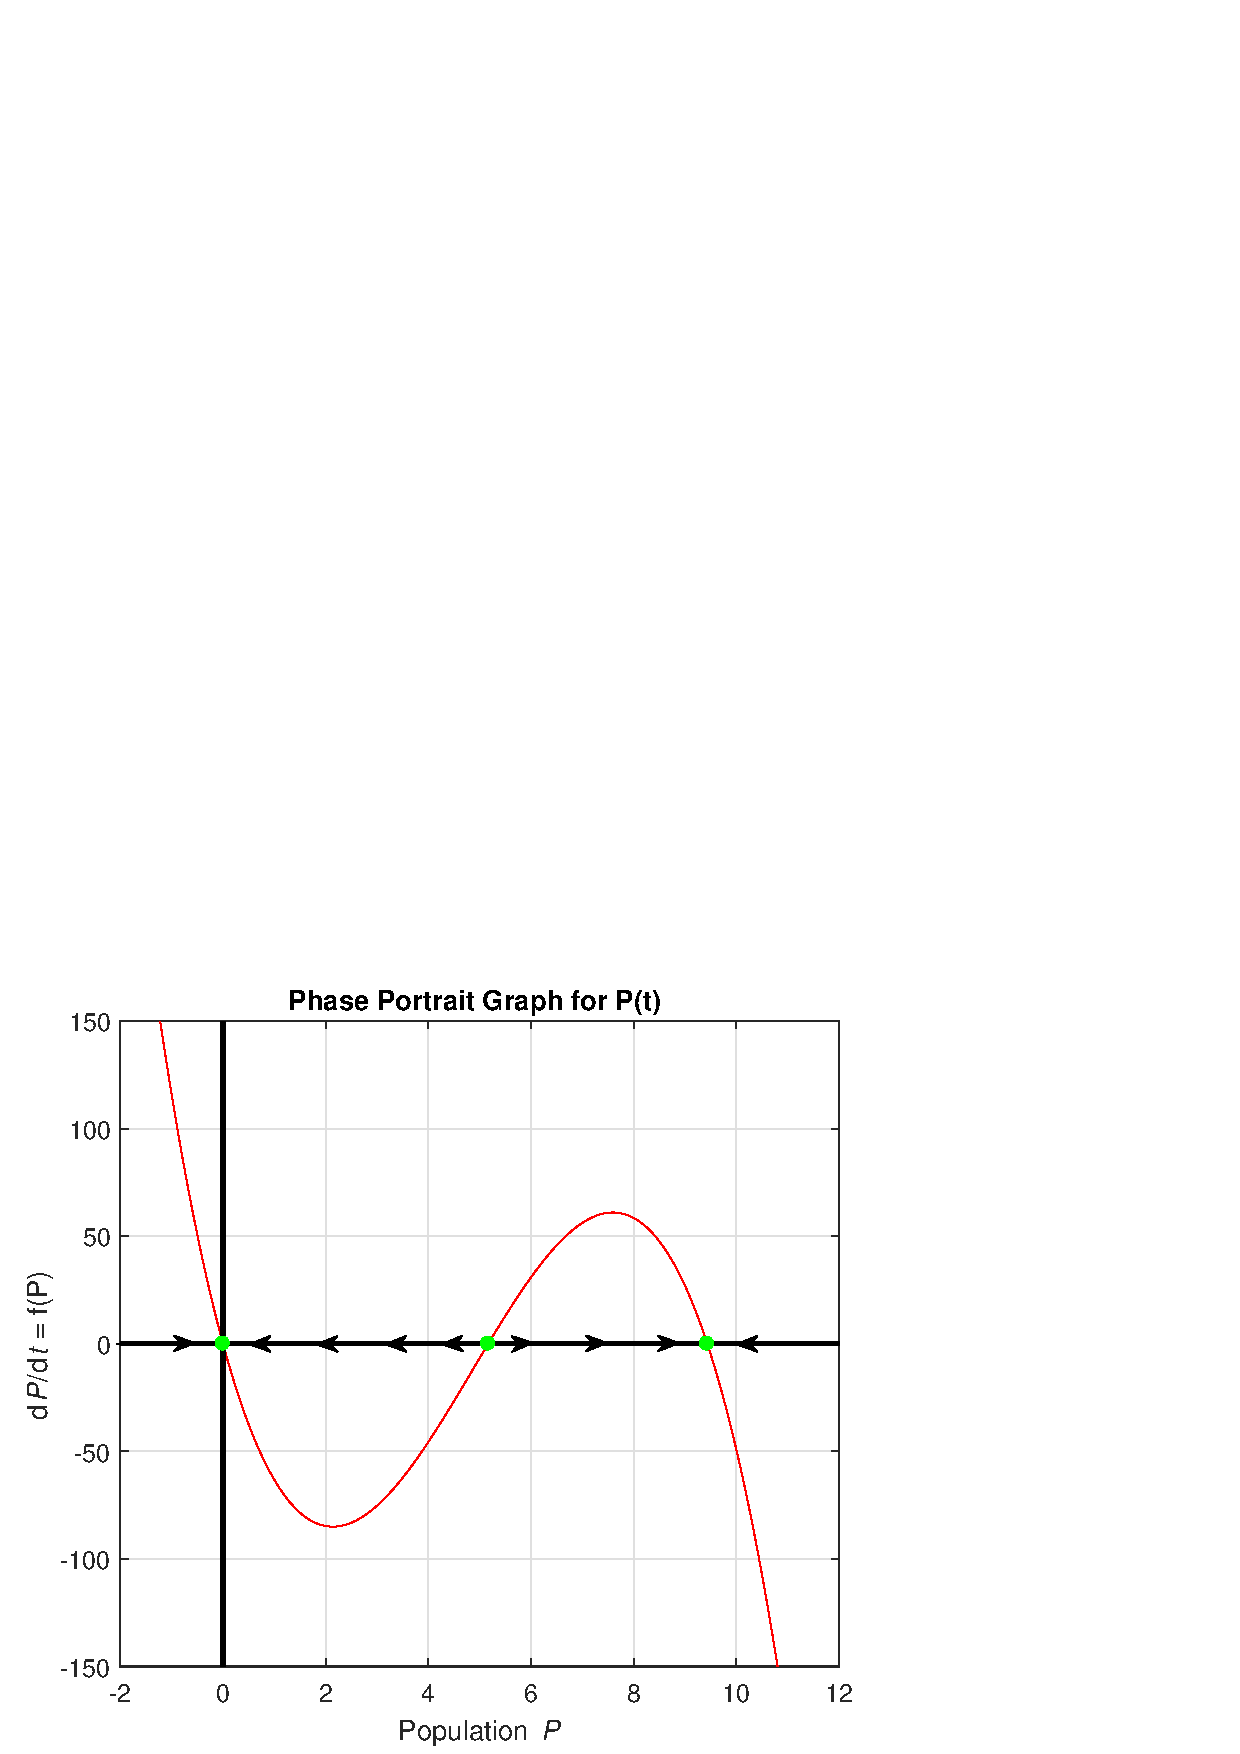
\includegraphics[width=13cm]{f6.png}}
	\centering{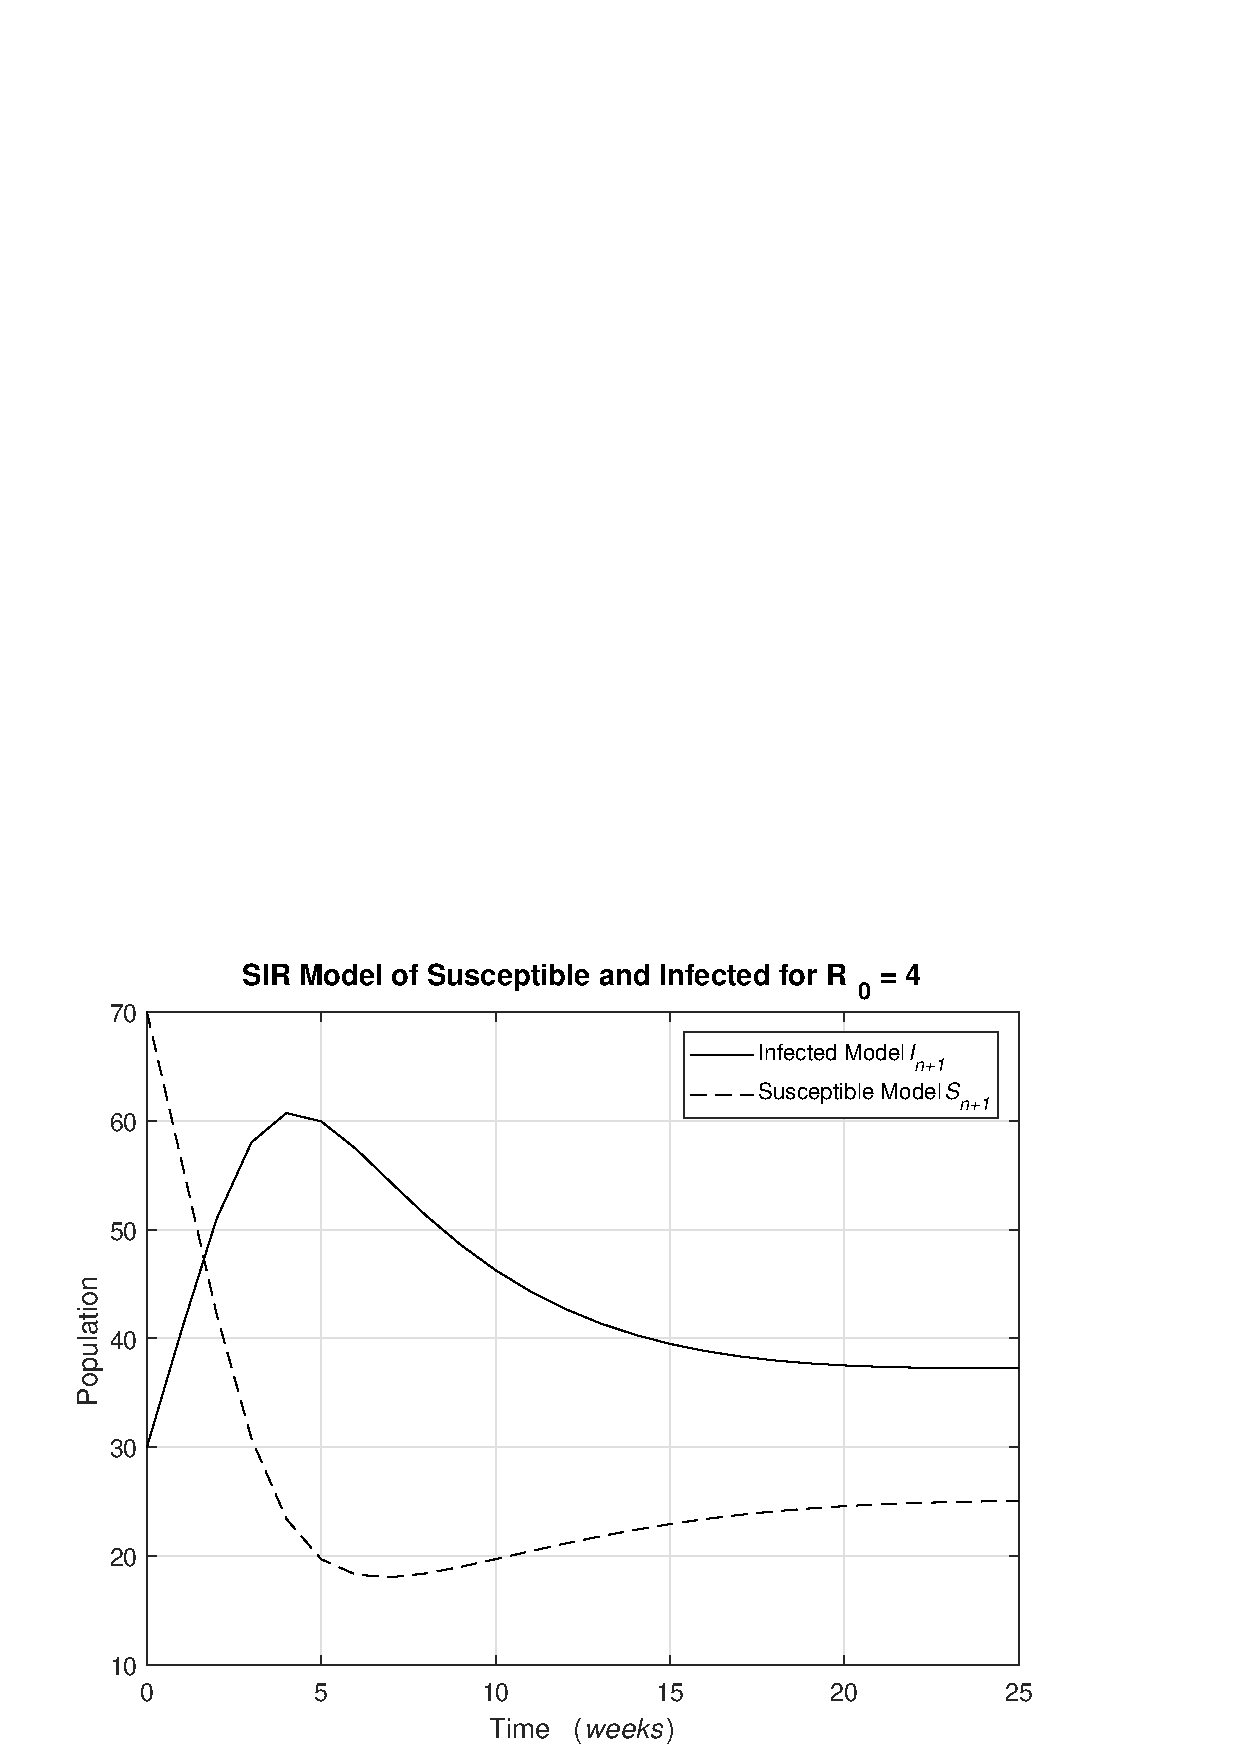
\includegraphics[width=13cm]{f5.png}}
	\caption*{\textbf{Figure ii} MATLAB Code for $dde23()$ Execution}
\end{figure}

\end{document}





































